Resumen de diferentes partes: 

- Ajuste de agentes -> LoRa? 
- El protocolo MCP
- El estado del arte en arquitecturas de agentes LLM y sistemas RAG
- El estado del arte en agentes integrados a proyectos software
- Redes neuronales?

2. Agentes LLM (Fundamentos y funcionamiento básico)

¿Qué son los agentes LLM?
2.1. Modelos LLM
2.2. Interacción con herramientas
2.3. Abstracciones en frameworks

\section{Agentes LLM}

Los agentes de Inteligencia Artificial son programas informáticos que implementan modelos computacionales avanzados para ejecutar diversas funciones específicas del contexto en el que se aplican. Tras siete décadas y media de investigación, los esfuerzos en el campo se han focalizado en agentes basados en Grandes Modelos de Lenguaje (LLM). 

\subsection{Modelos LLM}

Los modelos de lenguaje (LM) constituyen sistemas computacionales especializados en el procesamiento del lenguaje natural. Entre estos, destacan los grandes modelos de lenguaje, diseñados para acometer tareas  como la clasificación y generación de contenido lingüístico. Su fundamento técnico reside en redes neuronales que implementan la arquitectura Transformer [Attention is All You Need]. Para comprender el funcionamiento de dicha arquitectura, resulta imprescindible asimilar previamente conceptos como la tokenización y las representaciones vectoriales del lenguaje.

\paragraph{Tokens}
Los tokens constituyen la unidad mínima de texto que el modelo puede procesar. Dado que operan sobre estructuras matemáticas, requieren transformar el lenguaje natural en representaciones matriciales. Para lograr esta conversión, el texto se segmenta en dichas unidades mínimas, que pueden corresponder a caracteres individuales, fragmentos de texto o palabras completas. El conjunto íntegro de estas unidades reconocibles por el modelo configura su vocabulario. 

\paragraph{Representaciones vectoriales}
Constituyen vectores numéricos de dimensionalidad fija que codifican la semántica inherente a cada token. Estos vectores pueden comprender desde 768 dimensiones en arquitecturas como BERT-base hasta superar las 16.000 dimensiones en los modelos más avanzados del estado del arte, capturando conceptos semánticos en profundidad. Dichas representaciones se adquieren mediante procesos de aprendizaje durante la fase de entrenamiento del modelo. Por ejemplo, una dimensión específica podría especializarse en representar conceptos abstractos. En este contexto, la representación vectorial del token ``animal`` presentaría un valor más elevado en dicha dimensión que la correspondiente al término ``gato``, reflejando su mayor grado de abstracción conceptual.

\subsubsection{Arquitectura Transformer}
Esta arquitectura emplea el mecanismo de ``atención`` para enriquecer la comprensión textual del modelo. El proceso transforma inicialmente la representación de las palabras de entrada incorporando información contextual mediante múltiples capas de atención, que consisten en operaciones matriciales que transfieren información semántica entre palabras. 

Los agentes LLM utilizan predominantemente modelos decodificadores autorregresivos (GPT, Claude-Sonnet, Llama), optimizados para la generación secuencial de texto. Su característica distintiva es la aplicación de atención únicamente sobre tokens precedentes, permitiendo que el modelo compute la influencia de tokens anteriores sobre el actual sin modificar representaciones previas.

La figura \ref{fig:atencion_gato} ilustra un ejemplo simplificado del cómputo de atención para la frase ``El gato duerme``. Al generar la siguiente palabra, el modelo presta atención diferenciada a elementos previos, considerando más relevante que el gato esté durmiendo que su color. Así, calcula la probabilidad del siguiente token considerando todo el vocabulario disponible. Es importante destacar que, debido a la naturaleza autorregresiva, la influencia de un token posterior como ``negro`` no se aplica a tokens anteriores como ``gato``.

\begin{figure}
    \centering
    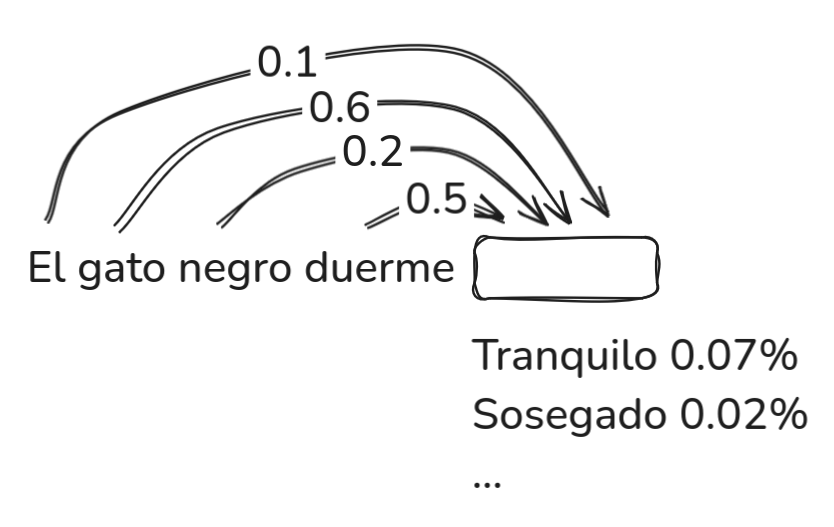
\includegraphics[width=0.65\linewidth]{figures/atencion_poc.png}
    \caption{Ejemplo simplificado de cómputo de atención para la frase \textquotedbl El gato duerme\textquotedbl}
    \label{fig:atencion_gato}
\end{figure}

En implementaciones prácticas, el mecanismo de atención que opera entre un token origen y un token destino se computa mediante operaciones matriciales que involucran tanto las representaciones vectoriales de ambos tokens como las matrices de atención, componentes de los parámetros aprendidos del modelo. Durante el proceso de entrenamiento, estas matrices de atención adquieren la capacidad de capturar fenómenos lingüísticos; por ejemplo, una matriz específica podría especializarse en cuantificar la connotación negativa que un token origen proyecta sobre un token destino.

\subsection{Interacción con herramientas externas}
Los agentes LLM tienen la capacidad de interactuar con múltiples herramientas como búsquedas en internet, interacciones con bases de datos, interacción con la interfaz de usuario, entre otras. A bajo nivel, un LLM no genera más que tokens de texto, por lo que la integración de herramientas se implementa mediante el uso de palabras clave que el modelo puede generar. Se le indica en el texto de entrada el esquema de la fucnión a utilizar, y de decidir utilizarla, el modelo generará el texto correspondiente a la función. Posteriormente se realizará una búsqeuda de expresiones regulares sobre la respuesta para obtener los datos necesarios para la ejecución de la función. 

La interacción con herramientas suele ser alternante. El modelo debe decidir si necesita utilizar una función, y en caso afirmativo, la salida de esta función se utilizará como entrada para el modelo. 

\subsection{Abstraciones en frameworks}
comentar lo de que se suele usar siempre una estructura conversacional, y que por eso suelen estar siempre ajustados para esta estructura, por lo que funcionan mejor así.










